\title{Computer Architecture - CS 301} % You may change the title if you want.

\author{Rishit Saiya - 180010027, Assignment - 14}

\date{\today}

\documentclass[12pt]{article}
\usepackage{fullpage}
\usepackage{enumitem}
\usepackage{amsmath,mathtools}
\usepackage{amssymb}
\usepackage[super]{nth}
\usepackage{textcomp}
\usepackage{hyperref}
\hypersetup{
    colorlinks=true,
    linkcolor=blue,
    filecolor=magenta,      
    urlcolor=cyan,
}
\begin{document}
\maketitle

%----------------------------------------------------------------

\section{}
\subsection{Storage Media}
If we turn off our system, all the data inside the processor and inside the memory devices like DRAM, etc. all of them get erased. But still files/data are intact with the system. The reason the data is unerased in because we have permanent data storage called Storage Media. Some examples of Storage Devices are Hard Disks, Optical Disks, Solid State Disks, etc.

\subsection{Hard Disk}
In this problem, we will focus on Hard Disk only. Hard Disk is a sequential magnetic arrangement that uses NRZI Encoding to store Data with the help of dummy bits. Figure 1 shows the NRZI Encoding used in Hard Disk. 
\begin{figure}
    \centering
    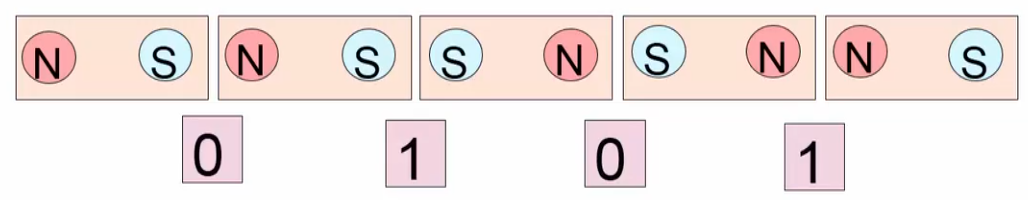
\includegraphics[width=12cm]{Assignment-14/NRZI.png}
    \caption{NRZI Encoding}
\end{figure}

\subsection{Addressing in Hard Disk}
The steps are followed as below. Hard Disks can also use this mechanism to mark bad sectors (sectors which are damaged permanently maybe lost its magnetic property) by storing information in recording surface about the sectors being good or bad, and then reconstruct the mapping between logical sectors and healthy physical sectors.
\begin{enumerate}
    \item The software programs use a component called Logical Block Address (LBA) to address a block in the hard disk. This might be alternatively referred as sector in the hard disk.
    \item The hard disk then internally converts the given logical address to a physical address. This physical address actually has the recording surface, track and sector information. 
    \item Most hard disk will dedicate a logical block which helps in recording surface for storing this information provided by the Logical Address.
    \item Hard Disks then use a small cache (DRAM) to store the most recently used mappings mapped from logical block to physical block.
    \item The hard disk can also use this mechanism to mark bad sectors and remap logical sectors to healthy physical sectors.
\end{enumerate}

%----------------------------------------------------------------

\section{}
A processing unit perceives a Hard Disk as a large array of bytes. But internally Hard Disk is fairly complex device and exposing such disks to Electro-Magnetic Field would lead to loss of data. Similarly hard disks also tend to have high failure rates because of high temperature sensitivity.

To mitigate our losses, we use RAID (Redundant Array of Disks) which are redundant disks and tolerate faults, and recover from failures RAID also helps to increase bandwidth and read from multiple disk in parallel. So our main idea is to safe guard our previous mapping onto a recording surface.

\subsection{Different Types of RAID Configurations}
\begin{itemize}
    \item \textbf{RAID 0:} \\
    In RAID 0 (Figure 2), we essentially have 2 disks. We store all the odd numbered blocks in one disk and all even numbered blocks in the other disk. This type of arrangement is known as Data Striping. \\
    It allows us to read even and odd blocks in parallel leading to increase in bandwidth in some cases. But if we want to read from data blocks that belong to same disk, then it won't be a case of bandwidth increase.
    Error coverage = No Reliability
    \begin{figure}
        \centering
        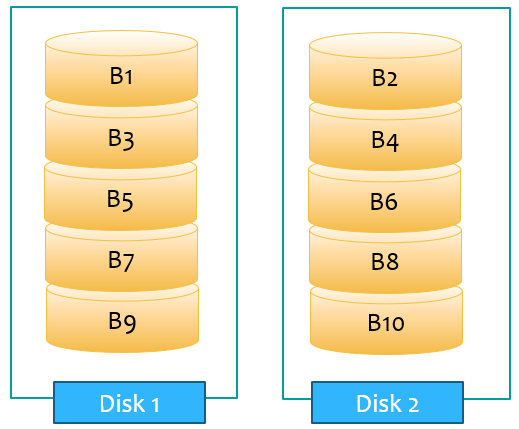
\includegraphics{Assignment-14/Raid_0.png}
        \caption{RAID 0}
    \end{figure}
    
    \item \textbf{RAID 1:} \\
    In RAID 1 (Figure 3), we again have 2 disks. The data blocks in Disk 1 are exactly replicated to constitute Disk 2, each block is of size 512 bytes. This can read blocks in parallel as it is mirror image of other disk. \\
    Error Coverage - Immune to just one disk failure. It means that if either disks fail, data can be recovered from functional disk. So, our bandwidth has doubled in this case. While data recovery, when a new disk is inserted after removing failed disk, all data can be copied to new disk from old functional disk by RAID software. 
    Overhead of the redundancy = 100\% overhead in storage.
    \begin{figure}
        \centering
        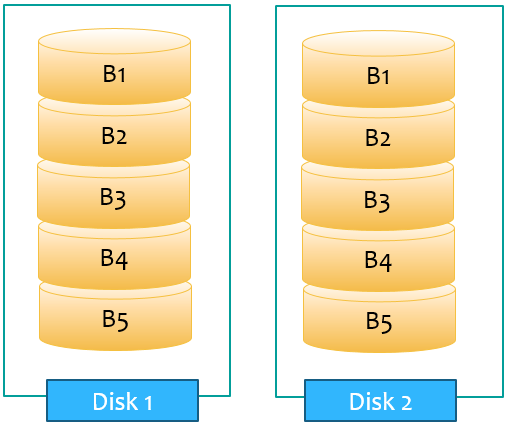
\includegraphics{Assignment-14/Raid_1.png}
        \caption{RAID 1}
    \end{figure}
    
    \item \textbf{RAID 2,3,4:} \\
    The RAID 2,3,4 belong to the same family of RAID protocols. In here we have a total of 5 disks, where 4 disks are for data storage and 1 disk is storing parity bits. As shown in Figure 5, small chunks of data are stored in blocks in Disk 1,2,3,4 and following XOR operation is performed to store corresponding Parity Block
    \begin{equation*}
        P1 = B1 \oplus B2 \oplus B3 \oplus B4
    \end{equation*}
    where P1 is the block in the Parity Disk.
    \begin{figure}
        \centering
        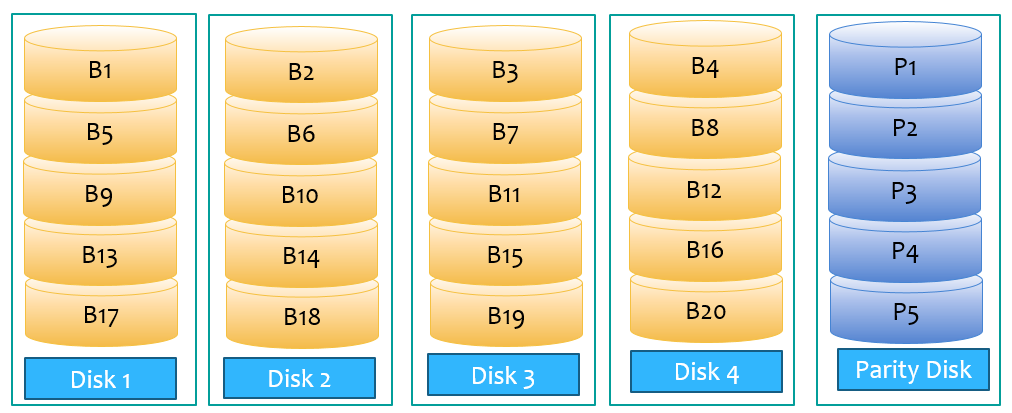
\includegraphics[width=15cm]{Assignment-14/Raid_234.png}
        \caption{RAID 2,3,4}
    \end{figure}
    In this case, if a disk fails, we can add a new disk and reconstruct our data back from the parity bits on data. Let's say that $B_1$ disk fails, then we can retrieve the data of $B_1$ by performing following XOR operation.
    \begin{equation*}
        B1 = P1 \oplus B2 \oplus B3 \oplus B4
    \end{equation*}
    Error Coverage - Immune to just one disk failure. If a disk fails, add a new disk and reconstruct it from the parity bits.
    Overhead of the redundancy = 25\% overhead in storage.
    The only problem with this RAID 4 is that for every read and write, we have to access Parity disk as well, thus parity disk becomes bottleneck. This problem is solved in RAID 5 which we will detail in below. The block size in RAID 2,3,4 is different and it is as follows (Table 1). \\
    % Table insert here:
    \begin{table}
    \centering
    \begin{tabular}{|c|c|} 
    \hline
    \textbf{RAID} & \textbf{Block Size}  \\ 
    \hline
    2             & 1 Bit                \\ 
    \hline
    3             & 1 Byte               \\ 
    \hline
    4             & 1 Block (512 Byte)   \\
    \hline
    \end{tabular}
    \caption{Block Size - RAID 2,3,4}
    \end{table}
    In RAID 2, we in general do not access data in the form of bits. So the access of data becomes bit complicated, which is why the usage is forfeited. In RAID 3, we have to write in many blocks for a small chunk of data which leads to increase in traffic, which is why this also proves to be less practical in implementation.
    
    \item \textbf{RAID 5:} \\
    In RAID 5 (Figure 5), we in general have 5 disks and instead of having a separate parity disk like in RAID 4, we distribute the parity blocks across the data storage disks. Distributing the parity blocks like this helps us to mitigate the issue of Parity Disk Failure and hence Data Retrieval is quicker.The storage overhead here will be same as in RAID 4. Additionally reliability also increases. The bandwidth increases upto 5 fold unless 2 request traffic are to the same disk. This system proves to be rather reliable.
    \begin{figure}
        \centering
        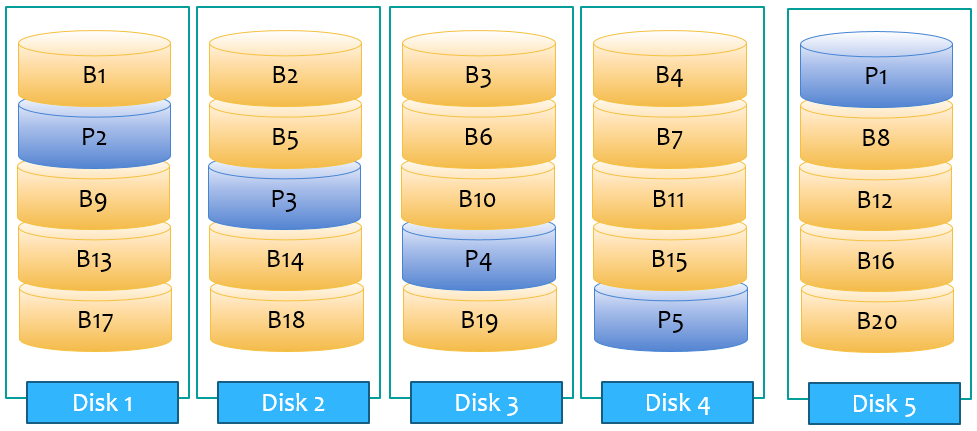
\includegraphics[width=15cm]{Assignment-14/Raid_5.png}
        \caption{RAID 5}
    \end{figure}
    
    
    \item \textbf{RAID 6:} \\
    In RAID 6 (Figure 6), we have 2 parity blocks per row where the parity blocks are rotated like in RAID 5 and are computed separately. Thus if memory is not an issue, RAID-6 is best possible configuration in terms of error coverage as it is immune to 2 disk failures.\\
    In here the Error Coverage - Immune to 2 disk failure. This instills high reliability but with a trade off with the cost of increase in overhead of  data storage.
    
    \begin{figure}
        \centering
        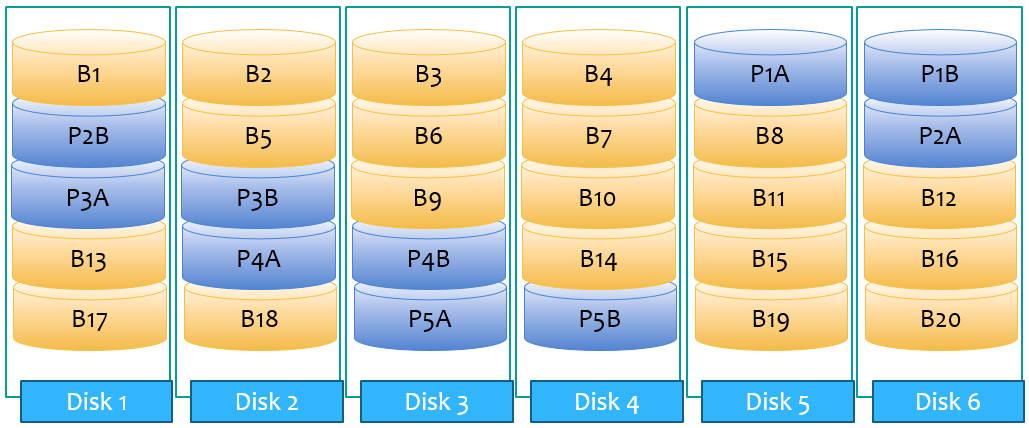
\includegraphics[width=15cm]{Assignment-14/Raid_6.png}
        \caption{RAID 6}
    \end{figure}
\end{itemize}
%----------------------------------------------------------------
\end{document}